\chapter{Entwurf} \label{chap:entwurf}
\section{Architektur der Datenbank} \label{sec:DB}
\begin{figure}[ht]
    \centering
    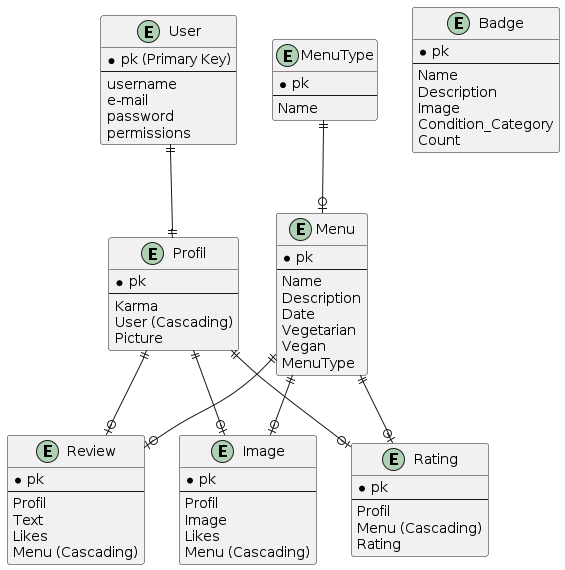
\includegraphics[width=0.8\textwidth]{images/Database.png}
    \caption{Architektur der Datenbank siehe auch \ref{code:core.models.py}}
    \label{fig:DB}
\end{figure}

Diese Skizze repräsentiert den Aufbau der Datenbank. Sie zeigt die verschiedenen
Entitiys und ihre Beziehungen. Die Datenbankstruktur ist in der Datei
\code{core/models.py} beschrieben (siehe \ref{code:core.models.py}).
